\chapter{Schwarze Löcher, weiße Löcher und das globale Kausaldiagramm}

\lectureoverview{Ein Horizont ist lokal gewöhnlich und global entscheidend. Wir beginnen mit der Schwarzschild-Metrik nahe dem Horizont, verfolgen sie mithilfe der Analogie zur euklidischen Zigarre nach außen und fragen dann, was Alice und Bob tatsächlich sehen können. Die Singularität und der zeitumgekehrte Bereich des weißen Lochs erweitern dieses lokale Bild zur ewigen Schwarzschild-Raumzeit. Durch die Penrose-Kompaktifizierung wird die Kausalstruktur endlich und übersichtlich. Im letzten Schritt wenden wir uns von einer ewigen Lösung einem durch Kollaps entstandenen schwarzen Loch zu; Newtons Schalensatz und Birkhoffs Theorem liefern die Teile, die zusammengefügt werden müssen.}

\section{Vom Horizont bis ins Unendliche}

In der Nähe eines hinreichend großen Schwarzschild-Horizonts ist die Krümmung auf der Skala eines kleinen Labors schwach, und die Geometrie von Radius und Zeit ist näherungsweise flach. Die zweckmäßige Radialkoordinate ist nicht die Schwarzschild-Koordinate \(r\), sondern der Eigenabstand \(\rho\), gemessen auf einer räumlichen Scheibe konstanter Zeit vom Horizont nach außen:
\begin{equation}
\rho=0 \quad\Longleftrightarrow\quad r=2GM .
\label{eq:l04-rho-horizon}
\end{equation}
Die zweckmäßige Zeitkoordinate ist die dimensionslose Größe
\begin{equation}
\omega=\frac{t}{4GM},
\label{eq:l04-omega}
\end{equation}
wobei \(c=1\) gilt. Somit ist \(\omega\) die Schwarzschild-Zeit, gemessen in Einheiten des doppelten Schwarzschild-Radius.

In der Vorzeichenkonvention mit überwiegend positiven Vorzeichen lautet die Metrik in radialer Richtung und Zeit nahe dem Horizont
\begin{equation}
ds^2\approx-\rho^2d\omega^2+d\rho^2.
\label{eq:l04-rindler}
\end{equation}
Die zweidimensionale Winkelsphäre ist hier unterdrückt, da die vorliegende Argumentation nur Zeit und Radialabstand betrifft.

\begin{figure}[htbp]
\centering
\includegraphics[width=0.72\textwidth]{lecture_04_figure_02.png}
\caption{Die Metrik nahe dem Horizont und die skalierte Schwarzschild-Zeit.}
\lectureframe{00:05:46.800}
\end{figure}

Gleichung~\eqref{eq:l04-rindler} steht in derselben Beziehung zur Minkowski-Raumzeit wie Polarkoordinaten zur euklidischen Ebene. Für
\begin{equation}
T=\rho\sinh\omega,
\qquad
X=\rho\cosh\omega,
\end{equation}
erhält man
\begin{equation}
-dT^2+dX^2=-\rho^2d\omega^2+d\rho^2.
\end{equation}
Linien konstanten \(\rho\) sind Hyperbeln \(X^2-T^2=\rho^2\), während \(\omega\) von der fernen Vergangenheit bis in die ferne Zukunft läuft. Die beiden lichtartigen Linien \(X=\pm T\) treffen sich im reduzierten Diagramm im Bifurkationspunkt. In vier Dimensionen entspricht dieser Punkt einer zweidimensionalen Sphäre; die zukünftige und die vergangene lichtartige Fläche bilden zusammen einen bifurkaten Killing-Horizont.\editorialnote{Im radialen Diagramm ist es als Kurzform nützlich, nur den Schnittpunkt als bifurkaten Horizont zu bezeichnen. Genauer gesagt schneiden sich die beiden Horizontäste auf einer Bifurkationssphäre.}

\subsection{Der Fernbereich}

Der radiale Anteil der Schwarzschild-Metrik lautet
\begin{equation}
ds^2
=-\left(1-\frac{2GM}{r}\right)dt^2
+\frac{dr^2}{1-\frac{2GM}{r}}.
\label{eq:l04-schwarzschild}
\end{equation}
Weit vom Loch entfernt, bei \(r\gg2GM\), nähert sich die Metrik der Form
\begin{equation}
ds^2\approx-dt^2+dr^2.
\end{equation}
Dort unterscheiden sich \(r\) und \(\rho\) nur durch eine unwesentliche additive Korrektur. Mit \(dt=4GM\,d\omega\) gilt daher
\begin{equation}
ds^2\approx-(4GM)^2d\omega^2+d\rho^2.
\label{eq:l04-far}
\end{equation}
Der Radialkoeffizient ist in beiden Grenzfällen einfach. Es ist der Zeitkoeffizient, der sich ändert:
\begin{equation}
ds^2\approx
\begin{cases}
-\rho^2d\omega^2+d\rho^2, & \rho\ll GM,\\[3pt]
-(4GM)^2d\omega^2+d\rho^2, & \rho\gg GM.
\end{cases}
\label{eq:l04-two-limits}
\end{equation}
Auf einer Bahn mit konstantem Radius gilt \(d\rho=0\). Nahe am Horizont ist
\begin{equation}
d\tau=\rho\,d\omega,
\end{equation}
weit entfernt dagegen \(d\tau\approx4GM\,d\omega=dt\). Für ein festes Zeitintervall der äußeren Zeitkoordinate vergeht auf einer Uhr umso weniger Eigenzeit, je näher sie am Horizont gehalten wird.

\subsection{Die Zigarre}

Raumzeit lässt sich schwer veranschaulichen; deshalb ersetzen wir die zeitartige Richtung durch eine gewöhnliche Winkelrichtung. Wir schreiben
\begin{equation}
\begin{aligned}
d\ell^2&=F(\rho)^2d\theta^2+d\rho^2,\\
F(\rho)&\sim
\begin{cases}
\rho, & \rho\to0,\\
4GM, & \rho\to\infty.
\end{cases}
\end{aligned}
\label{eq:l04-cigar}
\end{equation}
In der Nähe von \(\rho=0\) ist dies die Ebene in Polarkoordinaten. Weit entfernt wächst der Umfang nicht mehr mit dem Radius:
\begin{equation}
C_\infty=\int_0^{2\pi}4GM\,d\theta=8\pi GM.
\label{eq:l04-cigar-circumference}
\end{equation}
Die Fläche rundet sich somit an einem Ende ab und geht am anderen in einen Zylinder über. Sie sieht aus wie eine Zigarre.

\begin{figure}[htbp]
\centering
\includegraphics[width=0.74\textwidth]{lecture_04_figure_03.png}
\caption{Der euklidische Vergleich: eine polare Spitze, die in einen asymptotischen Zylinder mit Umfang \(8\pi GM\) übergeht.}
\lectureframe{00:14:05.000}
\end{figure}

Je größer die Masse, desto größer der asymptotische Umfang und desto sanfter die Krümmung nahe der Spitze. Ein kleines Loch entspricht einer eng gekrümmten Zigarre; bei einem großen Loch ist die Spitze breit und schwach gekrümmt. Dies veranschaulicht die Interpolation in Gleichung~\eqref{eq:l04-two-limits}, nicht aber eine Einbettung des Lorentzschen schwarzen Lochs selbst.\editorialnote{Das präzise geometrische Objekt erhält man, indem man die Schwarzschild-Zeit zur imaginären Zeit fortsetzt. Die Glattheit an der Spitze legt dann die Periode der euklidischen Zeit auf \(8\pi GM\) fest, also auf dieselbe Skala, die später die Hawking-Temperatur bestimmt. In dieser Vorlesung dient das Bild hier nur der Veranschaulichung.}

\section{Den Horizont kausal verstehen}

Außerhalb des Lochs, bei \(\rho>0\), bewegt sich ein ruhender Beobachter entlang einer Hyperbel konstanten \(\rho\). Weit entfernt genügt eine mäßige Beschleunigung, um der Gravitation entgegenzuwirken; nahe am Horizont wächst die erforderliche Eigenbeschleunigung unbegrenzt. Sobald eine Weltlinie die zukünftige lichtartige Grenze überschreitet, kann kein zukünftiges kausales Signal von ihr das Außen erreichen.

\begin{classroomqa}
\audiencequestion{Sind Lichtstrahlen in diesem Diagramm gerade Linien?\lecturetimestamp{00:20:21}}
\lecturerresponse{Radiale Lichtstrahlen werden unter einem Winkel von \(45^\circ\) eingezeichnet, sofern keine andere Konvention angegeben ist. Ein einfallender Strahl überschreitet den Horizont; ein auslaufender Strahl, der sich bereits im Inneren befindet, kann nicht wieder ins Außen gelangen.}
\end{classroomqa}

\begin{classroomqa}
\audiencequestion{Bleibt ein einfallender Lichtstrahl auf dem Horizont?\lecturetimestamp{00:21:12}}
\lecturerresponse{Nein. Ein nach innen gerichteter Strahl überschreitet den zukünftigen Horizont und setzt seinen Weg ins Innere des schwarzen Lochs fort. Nur ein Horizontgenerator selbst bleibt auf der lichtartigen Grenze.}
\end{classroomqa}

\subsection{Bob beobachtet Alice}

Bob halte sich bei festem Radius außerhalb auf, während Alice nach innen fällt. Er sieht Alice nur, indem er von ihr ausgehendes Licht empfängt. Nehmen wir an, sie winkt regelmäßig nach ihrer eigenen Uhr. Später während ihres Falls ausgesandte Signale benötigen immer mehr Schwarzschild-Zeit, um Bob zu erreichen, und er empfängt weniger Wellen pro Zeiteinheit. Kein Signal, das nach dem Überschreiten des Horizonts ausgesandt wird, kann zu ihm zurückkehren.

Die Rindler-Koordinaten machen das Grenzverhalten deutlich. Wir definieren die auslaufende lichtartige Koordinate
\begin{equation}
U=T-X=-\rho e^{-\omega}.
\end{equation}
Die Annäherung an den zukünftigen Horizont bedeutet \(U\to0^{-}\); bei festem äußeren \(\rho\) erfordert dies \(\omega\to+\infty\). Ein Ereignis, bei dem Alice den Horizont in endlicher Zeit überschreitet, wird daher auf unendliche äußere Zeit verschoben. Aufeinanderfolgende Wellenberge treffen mit exponentiell zunehmendem Abstand ein, sodass ihre Frequenz exponentiell rotverschoben wird.\editorialnote{Diese Rechnung mit der lichtartigen Koordinate liefert die mathematische Form der Rotverschiebung, die im Unterricht qualitativ beschrieben wurde. Sie verwendet nur die lokale Rindler-Näherung.}

Zunächst empfängt Bob sichtbares Licht, dann Infrarotstrahlung und schließlich Radiowellen mit enormer Wellenlänge. Die treffende Aussage ist nicht, dass Alice als dauerhaft sichtbares Foto auf dem Horizont verbleibt. Sie wird lichtschwächer und röter und schließlich unsichtbar.

\begin{classroomqa}
\audiencequestion{Sieht Bob Alice an einem exakt festgelegten Ort außerhalb des Horizonts erstarren?\lecturetimestamp{00:26:31}}
\lecturerresponse{In der klassischen Beschreibung mit äußeren Koordinaten stammen die zu immer späteren Zeiten empfangenen Bilder von Ereignissen, die immer näher am Horizont liegen. Das Grenzbild ist dort eingefroren, doch seine Strahlung wird so stark rotverschoben, dass es praktisch verschwindet. Quantenphysik schwarzer Löcher ist in dieser Darstellung noch nicht berücksichtigt.}
\end{classroomqa}

\begin{classroomqa}
\audiencequestion{Wirkt Alice beim Verblassen auch gestaucht?\lecturetimestamp{00:28:34}}
\lecturerresponse{Ja. Die Relativbewegung bewirkt in der äußeren Beschreibung eine Lorentz-Kontraktion in Längsrichtung. Der entscheidende Beobachtungseffekt ist hier weiterhin die Rotverschiebung: Ihre inneren Schwingungen erscheinen langsamer, und die empfangene Wellenlänge nimmt zu.}
\end{classroomqa}

\subsection{Alice beobachtet Bob}

Alices Eigenzeit verläuft am Horizont ganz regulär. Auch nach dem Überschreiten des Horizonts empfängt sie weiterhin einfallende Signale von Bob, denn diese bewegen sich in derselben Kausalrichtung wie sie. Sobald sie sich im Inneren befindet, kann sie dem Außen nicht mehr antworten. Der Horizont ist eine Einbahnstraße und keine Wand, die von beiden Seiten symmetrisch angetroffen wird.

\begin{classroomqa}
\audiencequestion{Sieht Alice Bobs Licht während ihres Falls blauverschoben?\lecturetimestamp{00:30:29}}
\lecturerresponse{In dem hier verwendeten Bild sieht sie, wie Bob sich entfernt, und seine Signale sind ins Rote verschoben; beim Überschreiten des Horizonts geschieht nichts Singuläres. Die genaue Frequenzverschiebung hängt von beiden Weltlinien und davon ab, wann Bob das Signal aussendet. Die invariante Aussage lautet daher, dass die von Alice gemessene Frequenz an einem regulären Horizont endlich bleibt.}
\end{classroomqa}

\begin{classroomqa}
\audiencequestion{Gilt dieselbe kausale Einschränkung auch für Gravitonen?\lecturetimestamp{00:31:15}}
\lecturerresponse{Sie gilt für echte Gravitationsstrahlung genauso wie für Photonen. Keine von hinter dem zukünftigen Horizont ausgesandte Strahlungsstörung kann Bob erreichen.}
\end{classroomqa}

\begin{classroomqa}
\audiencequestion{Erhöht Alices Energie die Masse und den Radius des Lochs, wenn sie hineinfällt?\lecturetimestamp{00:31:43}}
\lecturerresponse{Ja. Sobald ihre Energie zum schwarzen Loch gehört, nimmt dessen Masse zu, und sein Schwarzschild-Radius \(R_s=2GM\) wächst entsprechend. Das Problem der dynamischen Entstehung wird diese Aussage geometrisch fassen.}
\end{classroomqa}

\subsection{Warum das Außen dennoch Gravitation aufweist}

Ein schwarzes Loch ist dunkel, aber nicht gravitationsfrei. Ein stationäres Gravitationsfeld ist kein Strom von Schalen-Gravitonen, die fortwährend aus dem Inneren entweichen. Es ist die bereits etablierte äußere Geometrie. Ändert sich die Quelle, breitet sich die Änderung des Feldes kausal aus; ein weit entfernter Beobachter kann diese Änderung nicht feststellen, bevor ein Lichtsignal ihn erreichen könnte.

\begin{classroomqa}
\audiencequestion{Wenn Gravitonen nicht entkommen können, warum übt das schwarze Loch dann überhaupt Gravitation aus?\lecturetimestamp{00:32:04}}
\lecturerresponse{Das statische Feld ist außen bereits vorhanden. Man kann es umgangssprachlich mithilfe virtueller Gravitonen beschreiben, doch das sind keine nachweisbaren Teilchen, die neue Botschaften aus dem Inneren überbringen. Die Lichtgeschwindigkeit begrenzt die Ausbreitung einer Feldänderung, einschließlich der Gravitationsstrahlung.}
\end{classroomqa}

\begin{classroomqa}
\audiencequestion{Wie lassen sich virtuelle Gravitonen mit der Aussage vereinbaren, dass sich eine Feldänderung mit Lichtgeschwindigkeit ausbreitet?\lecturetimestamp{00:34:02}}
\lecturerresponse{Virtuelle Quanten sind Hilfsmittel der Buchführung in einer störungstheoretischen Rechnung und keine signalübertragenden Teilchen mit messbaren Bahnen. Eichinvariante Störungen und Information breiten sich kausal aus. Dieselbe Unterscheidung besteht zwischen einem statischen elektromagnetischen Feld und elektromagnetischer Strahlung.}
\end{classroomqa}

Die Aussage im Unterricht, virtuelle Gravitonen könnten sich schneller als Licht bewegen, ist daher nicht als überlichtschnelle Kommunikation zu verstehen.\editorialnote{Virtuelle Teilchen außerhalb der Massenschale müssen nicht die Dispersionsrelation für Teilchen auf der Massenschale erfüllen; sie sind jedoch keine Observablen und können nicht zur Informationsübertragung verwendet werden. In der allgemeinen Relativitätstheorie ist die klare Beschreibung einfacher: Die stationäre äußere Metrik besteht, während sich Änderungen des Gravitationsfelds kausal ausbreiten.}

\section{Kann Alice noch ihre Füße sehen?}

Alice falle mit den Füßen voran. Ihre Füße überschreiten den Horizont, bevor ihr Kopf ihn erreicht. Wenn sie nach unten blickt, sieht sie niemals das gleichzeitige Ereignis auf der Weltlinie ihrer Füße; Licht braucht Zeit, um sich auszubreiten, daher sieht sie ihre Füße bei einem etwas früheren Ereignis. Vor und nach dem Überschreiten des Horizonts durch ihren Kopf gibt es eine stetige Folge solcher vergangenen Ereignisse. Allein dadurch, dass ein Teil ihres Körpers \(r=2GM\) bereits passiert hat, geschieht lokal nichts Unstetiges.

Das gefährliche Gedankenexperiment besteht darin, den Kurs umzukehren, nachdem die Füße den Horizont überschritten haben. Um ihren Kopf außerhalb zu halten, muss Alice nach außen beschleunigen. Ihre Füße können, da sie sich bereits jenseits des zukünftigen Horizonts befinden, keiner schwebenden Bahn im Außen folgen. Im beschleunigten Bezugssystem wächst der Abstand unbegrenzt, und ein materieller Körper kann über diese kausale Grenze hinweg nicht starr bleiben. Alice muss entweder zusammen mit ihren Füßen frei fallen oder wird auseinandergerissen, wenn sie versucht, den übrigen Körper außerhalb zu halten.

Diese Dehnung ist keine divergierende Gezeitenkraft an einem großen Horizont. Sie ist die Folge der Forderung nach unvereinbaren Weltlinien für einen ausgedehnten Körper.\editorialnote{Ein hinreichend großer Schwarzschild-Horizont weist nur geringe Gezeitenkrümmung auf. Die Pathologie in diesem Gedankenexperiment entsteht durch den Versuch, Beschleunigung und Starrheitsbedingung zugleich zu erzwingen, nicht durch eine lokale Krümmungssingularität am Horizont.}

\section{Die Singularität liegt in der Zukunft}

Kehren wir zu Gleichung~\eqref{eq:l04-schwarzschild} zurück. Außerhalb gilt
\begin{equation}
1-\frac{2GM}{r}>0,
\end{equation}
somit ist \(t\) in Schwarzschild-Koordinaten zeitartig und \(r\) raumartig. Im Inneren gilt
\begin{equation}
1-\frac{2GM}{r}<0,
\end{equation}
und die kausalen Rollen dieser Koordinaten sind vertauscht: Ein kleiner werdendes \(r\) weist in eine zeitartige Richtung. Das bedeutet nicht, dass sich der Raum am Horizont physisch in Zeit verwandelt. Es bedeutet, dass die Schwarzschild-Karte dort degeneriert und ihre Koordinatenbeschriftungen im Inneren einen anderen Kausalcharakter haben.

Die eigentliche Singularität liegt bei
\begin{equation}
r=0.
\end{equation}
Sie ist keine vertikale Weltlinie, die einen Ort darstellt, dem man ausweichen könnte. Sie ist eine raumartige zukünftige Grenze. Sobald Alice in den Bereich des schwarzen Lochs eintritt, endet dort jeder zukünftige zeitartige oder lichtartige Weg. Die Krümmungsinvariante
\begin{equation}
R_{\mu\nu\rho\sigma}R^{\mu\nu\rho\sigma}
=\frac{48G^2M^2}{r^6}
\label{eq:l04-kretschmann}
\end{equation}
divergiert für \(r\to0\), während sie bei \(r=2GM\) endlich ist.\editorialnote{Gleichung~\eqref{eq:l04-kretschmann} ist der übliche Kretschmann-Skalar für die Schwarzschild-Lösung. Sie macht den im Unterricht geometrisch erläuterten Unterschied zwischen dem regulären Horizont und der Krümmungssingularität invariant.}

\section{Zeitumkehr und das weiße Loch}

Die Schwarzschild-Metrik ist unabhängig von \(t\), und \(dt^2\) bleibt unter \(t\mapsto-t\) unverändert. Ihre maximale Erweiterung ist daher symmetrisch unter Zeitumkehr. Neben der zukünftigen Singularität und dem zukünftigen Horizont enthält die mathematische Lösung auch eine vergangene Singularität und einen vergangenen Horizont.

Kehren wir Alices Fall zeitlich um. Nun tritt sie aus der vergangenen Singularität hervor, überschreitet den vergangenen Horizont nach außen und erscheint in Bobs Außenbereich. Dieser Bereich wird weißes Loch genannt. Er ist kein Fluchtweg aus dem zukünftigen Inneren des schwarzen Lochs: Der zukünftige und der vergangene Horizont sind verschiedene lichtartige Grenzen.

\begin{classroomqa}
\audiencequestion{Wenn Alice den Horizont des schwarzen Lochs nicht nach außen überschreiten kann, wie kann dann die zeitlich umgekehrte Alice herauskommen?\lecturetimestamp{00:50:24}}
\lecturerresponse{Sie überschreitet nicht den zukünftigen Horizont nach außen. Sie überschreitet den vergangenen Horizont nach außen, genau wie es der Zeitumkehr eines gewöhnlichen Einfalls entspricht. Aus dem zukünftigen Bereich des schwarzen Lochs führt weiterhin kein kausaler Weg nach außen.}
\end{classroomqa}

\begin{classroomqa}
\audiencequestion{Muss im Bild des weißen Lochs auch Bobs gesamte Geschichte rückwärts ablaufen?\lecturetimestamp{00:52:15}}
\lecturerresponse{Nein. Die erweiterte Geometrie lässt eine Geschichte zu, in der Bob im Außenbereich bleibt, während Alice aus dem vergangenen Horizont hervortritt. Das Rätsel besteht nicht in der mathematischen Konsistenz, sondern in der außergewöhnlichen Anfangsbedingung, die durch die vergangene Singularität dargestellt wird.}
\end{classroomqa}

\begin{figure}[htbp]
\centering
\includegraphics[width=0.72\textwidth]{lecture_04_figure_04.png}
\caption{Die ausgearbeitete Kausalskizze: sich kreuzende Horizonte, zukünftige und vergangene Singularitätskurven sowie im Laufe der Diskussion ergänzte Beobachterbahnen.}
\lectureframe{01:00:19.818}
\end{figure}

\begin{figure}[htbp]
\centering
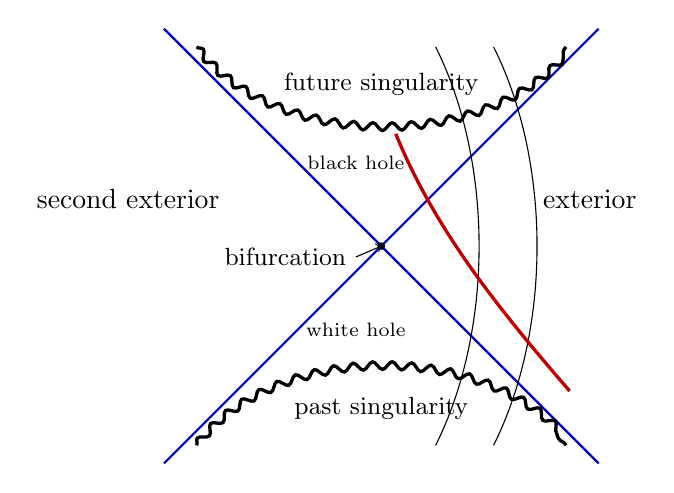
\begin{tikzpicture}[scale=0.92]
\draw[blue!75!black,thick] (-3,-3) -- (3,3);
\draw[blue!75!black,thick] (-3,3) -- (3,-3);
\draw[very thick,decorate,decoration={snake,amplitude=1.4pt,segment length=7pt}]
  (-2.55,2.75) .. controls (-1.45,1.35) and (1.45,1.35) .. (2.55,2.75);
\draw[very thick,decorate,decoration={snake,amplitude=1.4pt,segment length=7pt}]
  (-2.55,-2.75) .. controls (-1.45,-1.35) and (1.45,-1.35) .. (2.55,-2.75);
\draw (0.75,-2.75) .. controls (1.55,-1.15) and (1.55,1.15) .. (0.75,2.75);
\draw (1.55,-2.75) .. controls (2.35,-1.15) and (2.35,1.15) .. (1.55,2.75);
\draw[red!75!black,very thick] (2.6,-2.0) .. controls (1.65,-0.9) and (0.75,0.2) .. (0.2,1.55);
\fill (0,0) circle (1.5pt);
\node[above,font=\small] at (0,1.95) {future singularity};
\node[below,font=\small] at (0,-1.95) {past singularity};
\node[right] at (2.10,0.65) {exterior};
\node[left] at (-2.10,0.65) {second exterior};
\node[font=\scriptsize] at (-0.35,1.15) {black hole};
\node[font=\scriptsize] at (-0.35,-1.15) {white hole};
\node[font=\small,anchor=east] (bifurcation-label) at (-0.35,-0.15) {bifurcation};
\draw[->,thin] (bifurcation-label.east) -- (0,0);
\end{tikzpicture}
\caption{Eine bereinigte, nicht kompaktifizierte Kausalzeichnung. Die lichtartigen Horizonte schneiden sich auf der Bifurkationsfläche; die raumartigen Singularitäten liegen im zukünftigen und im vergangenen Keil.}
\end{figure}

\subsection{Möglich heißt nicht typisch}

Die mikroskopischen Gesetze sind mit sehr guter Näherung zeitumkehrinvariant, dennoch haben makroskopische Abläufe eine bevorzugte Richtung. Eine Bombe explodiert leicht; verstreute Trümmer finden fast nie wieder zusammen und setzen sich zur Bombe zusammen. Ein Ball rollt leicht von einem instabilen Gipfel hinab; ein zufällig geworfener Ball kommt fast nie genau dort zur Ruhe. Eine aufgestellte Reihe von Billardkugeln zerstreut sich leicht, während verstreute Kugeln sich nicht spontan wieder zu dieser Aufstellung ordnen. Ein Eiswürfel schmilzt in heißem Wasser, während das Wasser fast nie einen neu zusammengesetzten Eiswürfel ausstößt.

Der Unterschied liegt in der Entropie. Ein Makrozustand niedriger Entropie nimmt einen winzigen Bereich des Phasenraums ein; ein Makrozustand hoher Entropie umfasst eine ungeheure Zahl mikroskopischer Anordnungen. Die Gleichungen erlauben die umgekehrte Bahn, doch die dafür nötige präzise Korrelation des Anfangsmikrozustands wäre fantastisch genau herzustellen.

\begin{classroomqa}
\audiencequestion{Ist nicht jede exakt festgelegte Anordnung verstreuter Kugeln genauso unwahrscheinlich wie die exakt zeitumgekehrte Anordnung?\lecturetimestamp{00:56:55}}
\lecturerresponse{Ja, wenn man einzelne Mikrozustände genau vorgibt. Die Asymmetrie zeigt sich beim Vergleich von Makrozuständen. Eine verstreute Anordnung umfasst ungleich mehr Mikrozustände als ein präzise aufgestelltes Dreieck; daher bleibt fast jeder mit der ersten Beschreibung verträgliche mikroskopische Zustand makroskopisch ungeordnet.}
\end{classroomqa}

Ein weißes Loch, das eine vollständig geordnete Alice ausstößt, ist die gravitative Entsprechung eines solchen entropieverringernden Verlaufs. Er ist mit den umkehrbaren Gleichungen vereinbar, setzt aber eine außerordentlich spezielle Vergangenheit voraus. Der Horizont trägt selbst Entropie und verborgene mikroskopische Information; eine Fluktuation von der Größe Alices ist daher logisch nicht ausgeschlossen, aber überwältigend stark unterdrückt.

\begin{classroomqa}
\audiencequestion{Wäre eine solche Fluktuation quantenmechanisch oder thermisch?\lecturetimestamp{00:59:48}}
\lecturerresponse{Beide Arten können dazu beitragen. In einem gewöhnlichen heißen System spricht man vor allem von einer thermischen Fluktuation; bei einem schwarzen Loch sind Quanten- und thermische Effekte miteinander verflochten. In beiden Fällen ist die entscheidende Unterdrückung entropisch.}
\end{classroomqa}

\section{Eigenabstand und Penrose-Kompaktifizierung}

Bevor wir die globale Raumzeit zeichnen, sollten wir die Begriffe zum Radialabstand präzisieren. Die Eigenzeit ist das, was eine Uhr entlang einer zeitartigen Weltlinie misst. Der Eigenabstand ist das, was eine Kette lokaler Meterstäbe entlang einer gewählten raumartigen Kurve misst. Für die Schwarzschild-Scheibe mit konstantem \(t\) gilt
\begin{equation}
d\rho=\frac{dr}{\sqrt{1-2GM/r}}.
\label{eq:l04-proper-distance}
\end{equation}
Somit ist \(r\) eine Flächenradiuskoordinate und nicht der direkte Abstand vom Horizont, den ein Meterstab misst.

Beginnen wir nun mit radialer flacher Raumzeit. Behalten wir nur \(t\) und \(\rho\ge0\) bei. Die Linie \(\rho=0\) ist der räumliche Ursprung; ein radialer Lichtstrahl, der in den Ursprung eintritt, setzt sich auf der gegenüberliegenden physikalischen Seite nach außen fort, was in der reduzierten Halbebene als Reflexion erscheint.

Ein Penrose-Diagramm bildet alle endlichen und unendlichen Werte von \(t\) und \(\rho\) auf einen endlichen Bereich ab und erhält dabei die lichtartigen Richtungen. Es beruht auf zwei Regeln:
\begin{enumerate}
\item die gesamte Raumzeit auf einen endlichen Bereich kompaktifizieren;
\item radiale Lichtstrahlen bei \(45^\circ\) halten.
\end{enumerate}
Längen und gewöhnliche Winkel werden verzerrt; die Kausalbeziehungen bleiben erhalten.

\begin{figure}[htbp]
\centering
\includegraphics[width=0.70\textwidth]{lecture_04_figure_06.png}
\caption{Das vollständige Kompaktifizierungsraster für die radiale Minkowski-Raumzeit. Unendliche Zeiten liegen an den oberen und unteren Endpunkten links; der unendliche Radius ist auf die rechte Spitze zusammengedrückt.}
\lectureframe{01:14:44.040}
\end{figure}

\begin{figure}[htbp]
\centering
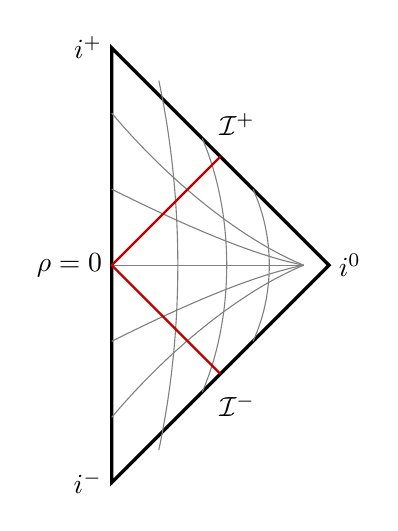
\begin{tikzpicture}[scale=0.92]
\coordinate (im) at (0,-3);
\coordinate (ip) at (0,3);
\coordinate (iz) at (3,0);
\draw[very thick] (im) -- (ip) -- (iz) -- cycle;
\draw[gray] (0,-2.1) .. controls (0.8,-1.15) and (1.8,-0.35) .. (2.65,0);
\draw[gray] (0,-1.05) .. controls (0.9,-0.6) and (1.9,-0.15) .. (2.65,0);
\draw[gray] (0,0) -- (2.65,0);
\draw[gray] (0,1.05) .. controls (0.9,0.6) and (1.9,0.15) .. (2.65,0);
\draw[gray] (0,2.1) .. controls (0.8,1.15) and (1.8,0.35) .. (2.65,0);
\draw[gray] (0.65,-2.55) .. controls (1.0,-0.9) and (1.0,0.9) .. (0.65,2.55);
\draw[gray] (1.25,-1.75) .. controls (1.7,-0.7) and (1.7,0.7) .. (1.25,1.75);
\draw[gray] (1.95,-1.05) .. controls (2.25,-0.4) and (2.25,0.4) .. (1.95,1.05);
\draw[red!75!black,thick] (1.5,-1.5) -- (0,0) -- (1.5,1.5);
\node[left] at (ip) {\(i^+\)};
\node[left] at (im) {\(i^-\)};
\node[right] at (iz) {\(i^0\)};
\node[above right] at (1.35,1.65) {\(\mathcal{I}^+\)};
\node[below right] at (1.35,-1.65) {\(\mathcal{I}^-\)};
\node[left] at (0,0) {\(\rho=0\)};
\end{tikzpicture}
\caption{Die radiale Minkowski-Raumzeit als endliches Dreieck. Der rote lichtartige Strahl tritt von \(\mathcal{I}^-\) ein, erreicht den Ursprung und verlässt ihn durch \(\mathcal{I}^+\).}
\label{fig:l04-flat-penrose}
\end{figure}

Die Endpunkte haben unterschiedliche kausale Bedeutungen:
\begin{equation}
\begin{aligned}
i^-&:\ \text{past timelike infinity},\\
i^+&:\ \text{future timelike infinity},\\
i^0&:\ \text{spatial infinity},\\
\mathcal{I}^-&:\ \text{past null infinity},\\
\mathcal{I}^+&:\ \text{future null infinity}.
\end{aligned}
\end{equation}
Die Symbole \(\mathcal{I}^{-}\) und \(\mathcal{I}^{+}\) werden „Scri minus“ und „Scri plus“ ausgesprochen.

\begin{classroomqa}
\audiencequestion{Müsste ein lichtartiger Strahl durch die Ecken jeder verzerrten Rasterzelle verlaufen und deshalb leicht gekrümmt sein?\lecturetimestamp{01:11:08}}
\lecturerresponse{Wenn das vollständige Koordinatenraster exakt eingezeichnet wäre, wären seine Schnittpunkte mit der lichtartigen Kurve vereinbar. Entscheidend ist die konforme Konstruktion: Radiale lichtartige Richtungen bleiben bei \(45^\circ\), auch wenn sich die Linien konstanten \(t\) und konstanten \(\rho\) krümmen und zusammendrängen.}
\end{classroomqa}

\begin{classroomqa}
\audiencequestion{Wie zeichnet man einen Lichtstrahl ein, wenn er den Ursprung verfehlt?\lecturetimestamp{01:11:45}}
\lecturerresponse{Er erreicht einen minimalen Abstand ungleich null und kehrt dann nach außen zurück. Berücksichtigt man die Winkelbewegung, muss seine projizierte radiale Bahn keine einzelne gerade Linie unter \(45^\circ\) sein.}
\end{classroomqa}

\begin{classroomqa}
\audiencequestion{Warum verläuft dieser Lichtstrahl dann nicht unter \(45^\circ\)?\lecturetimestamp{01:12:49}}
\lecturerresponse{Die Regel mit \(45^\circ\) wurde für radiale Lichtstrahlen formuliert. Ein lichtartiger Strahl mit Drehimpuls bewegt sich teilweise in den Winkelrichtungen; seine Projektion auf die \(t\)-\(\rho\)-Ebene ist daher nicht radial.}
\end{classroomqa}

\section{Das ewige Schwarzschild-Diagramm}

Das kompaktifizierte Diagramm hat vier Bereiche. Die beiden seitlichen Rauten sind asymptotisch flache Außenbereiche. Das obere Dreieck ist das Innere des schwarzen Lochs und endet an der zukünftigen raumartigen Singularität. Das untere Dreieck ist der Bereich des weißen Lochs und beginnt an der vergangenen raumartigen Singularität. Zusammen bilden diese Bereiche die maximal erweiterte Schwarzschild-Geometrie.

\begin{figure}[htbp]
\centering
\includegraphics[width=0.74\textwidth]{lecture_04_figure_07.png}
\caption{Das vollständige Penrose-Diagramm des ewigen Schwarzschild-Raums mit eingezeichneten Singularitäten, Horizonten, lichtartigen Bahnen und einer asymptotischen Grenze, wie es an der Tafel entstand.}
\lectureframe{01:21:30.000}
\end{figure}

\begin{figure}[htbp]
\centering
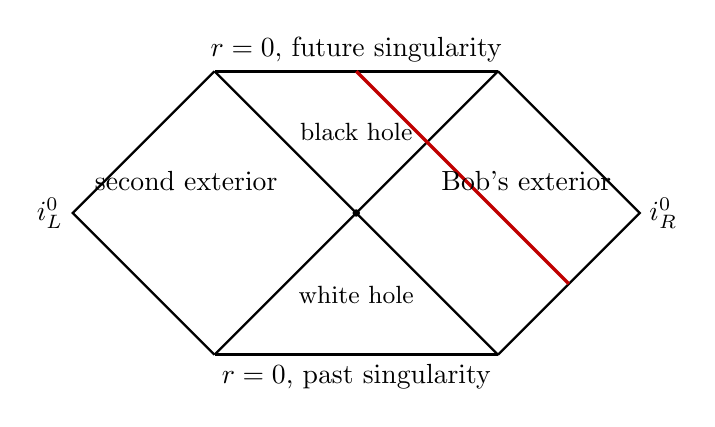
\begin{tikzpicture}[scale=0.90]
\coordinate (C) at (0,0);
\coordinate (TL) at (-2,2);
\coordinate (TR) at (2,2);
\coordinate (BL) at (-2,-2);
\coordinate (BR) at (2,-2);
\coordinate (L) at (-4.0,0);
\coordinate (R) at (4.0,0);
\draw[very thick] (TL) -- (TR);
\draw[very thick] (BL) -- (BR);
\draw[thick] (C) -- (TL) (C) -- (TR) (C) -- (BL) (C) -- (BR);
\draw[thick] (TL) -- (L) -- (BL);
\draw[thick] (TR) -- (R) -- (BR);
\draw[red!75!black,very thick] (3,-1) -- (1,1) -- (0,2);
\node[above] at (0,2) {\(r=0\), future singularity};
\node[below] at (0,-2) {\(r=0\), past singularity};
\node[font=\small] at (0,1.15) {black hole};
\node[font=\small] at (0,-1.15) {white hole};
\node at (2.4,0.45) {Bob's exterior};
\node at (-2.4,0.45) {second exterior};
\node[right] at (R) {\(i^0_R\)};
\node[left] at (L) {\(i^0_L\)};
\fill (C) circle (1.5pt);
\end{tikzpicture}
\caption{Die vier Bereiche des ewigen Schwarzschild-Raums. Ein einfallender radialer Lichtstrahl überschreitet den zukünftigen Horizont und endet bei \(r=0\).}
\label{fig:l04-eternal}
\end{figure}

Ein radialer einfallender Lichtstrahl von \(\mathcal{I}^-\) überschreitet den zukünftigen Horizont und endet an der Singularität. Jede kausale Kurve im oberen Dreieck hat dasselbe Schicksal. Der zweite Außenbereich wird oft als anderer Zugang zu einer Einstein--Rosen-Brücke beschrieben, doch diese ist nicht durchquerbar: Jeder versuchte kausale Weg von einem Außenbereich zum anderen führt in den Bereich des schwarzen Lochs und endet an der Singularität.

\begin{classroomqa}
\audiencequestion{Sind die beiden Außenwelten durch ein Wurmloch verbunden, und kann ein Signal hindurchgelangen?\lecturetimestamp{01:22:21}}
\lecturerresponse{Die ewige Geometrie enthält auf geeigneten räumlichen Scheiben eine Einstein--Rosen-Brücke, doch kein kausales Signal gelangt von einem Außenbereich zum anderen. Die Brücke schnürt sich zu schnell ab; selbst Licht, das einen Horizont überschreitet, endet an der zukünftigen Singularität.}
\end{classroomqa}

Dieses Diagramm beschreibt ein Loch, das schon immer existiert hat. Reale astrophysikalische Löcher entstehen durch kollabierende Materie. Ihr Kausaldiagramm enthält weder eine vergangene Singularität des weißen Lochs noch einen zweiten asymptotischen Außenbereich. Um diese Geometrie zu konstruieren, müssen wir sphärische Schalen verstehen.

\section{Ein schwarzes Loch durch Kollaps erzeugen}

Stellen wir uns eine diffuse sphärische Schale einfallender Teilchen vor. Es können Photonen sein: Energie gravitert, daher kann ein hinreichend konzentrierter Strahlungsimpuls ein schwarzes Loch bilden. Vor dem Kollaps ähnelt der zentrale Bereich leerer flacher Raumzeit; nachdem genügend Energie komprimiert wurde, ähnelt der Außenbereich der Schwarzschild-Geometrie. Die Aufgabe besteht darin, diese Bereiche über die bewegte Schale hinweg zusammenzufügen.

\subsection{Newtons Schalensatz}

Für eine kugelsymmetrische Newtonsche Schale der Gesamtmasse \(M\) lautet das Gaußsche Gesetz der Gravitation
\begin{equation}
\oint \mathbf{g}\cdot d\mathbf{A}=-4\pi G M_{\mathrm{enc}}.
\label{eq:l04-gauss-gravity}
\end{equation}
Aufgrund der Kugelsymmetrie gilt \(\mathbf{g}=g(r)\hat{\mathbf r}\), also
\begin{equation}
g(r)=
\begin{cases}
0, & r<R_{\mathrm{shell}},\\[4pt]
-\dfrac{GM}{r^2}, & r>R_{\mathrm{shell}}.
\end{cases}
\label{eq:l04-shell-field}
\end{equation}
Im Inneren ist keine Masse eingeschlossen, und das Gravitationsfeld verschwindet. Außerhalb wirkt die Schale exakt wie eine Punktmasse \(M\) im Zentrum. Das Potential im Inneren ist konstant, nicht null; eine lokale Newtonsche Kraft wirkt dort jedoch nicht.\editorialnote{Das im Unterricht erläuterte Argument mit den Feldlinien wird durch das Gaußsche Gesetz präzise wiedergegeben. Die Unterscheidung zwischen verschwindendem Feld und konstantem Potential ist beim Vergleich von Taktnormierungen in der Relativitätstheorie wichtig.}

Die Schlussfolgerung bleibt auch während des Zusammenziehens einer perfekt kugelförmigen Schale gültig, sofern ihre Gesamtmasse erhalten bleibt. Es ändert sich nur die Lage der Grenze zwischen der inneren und der äußeren Lösung.

\subsection{Birkhoffs Theorem}

Das relativistische Gegenstück ist Birkhoffs Theorem: Jeder kugelsymmetrische Vakuumbereich ist lokal ein Teil der Schwarzschild-Familie. Für eine Schale ohne Masse in ihrem Zentrum gilt
\begin{align}
ds^2_{\mathrm{inside}}&=-dT^2+dR^2+R^2d\Omega_2^2,\\
ds^2_{\mathrm{outside}}&=
-\left(1-\frac{2GM}{r}\right)dt^2
\nonumber\\
&\quad+\frac{dr^2}{1-2GM/r}
+r^2d\Omega_2^2.
\label{eq:l04-birkhoff-pieces}
\end{align}

\begin{figure}[htbp]
\centering
\includegraphics[width=0.74\textwidth]{lecture_04_figure_08.png}
\caption{Tafelbild zur Anpassung an der Schale: flache Raumzeit innerhalb des Kreises und die Schwarzschild-Lösung außerhalb.}
\lectureframe{01:34:15.000}
\end{figure}

\begin{classroomqa}
\audiencequestion{Welche Metrik liegt in der allgemeinen Relativitätstheorie außerhalb einer sphärischen Schale vor?\lecturetimestamp{01:33:17}}
\lecturerresponse{Die Schwarzschild-Metrik mit einem Massenparameter, der der erhaltenen Gesamtmasse der Schale entspricht. Der leere Zentralbereich ist lokal Minkowski-Raumzeit.}
\end{classroomqa}

\begin{classroomqa}
\audiencequestion{Wenn sich die Schale zusammenzieht, warum ändert sich dann der Massenparameter nicht?\lecturetimestamp{01:34:33}}
\lecturerresponse{Weil die Gesamtenergie erhalten bleibt. Radius, kinetische Energie und Bindungsenergie der Schale können sich ändern, doch die erhaltene Außenmasse eines isolierten kugelsymmetrischen Systems bleibt konstant. Durch die Bewegung der Schale ändert sich, wo der flache Bereich und der Schwarzschild-Bereich zusammengefügt werden.}
\end{classroomqa}

Eine flache Innenregion bedeutet nicht, dass eine Uhr im Inneren notwendigerweise dieselbe Normierung hat wie eine Uhr im Unendlichen. Die Anpassung über die Schale hinweg kann die innere Zeitkoordinate mit einer Konstanten multiplizieren, und bei einer bewegten Schale sind die entsprechenden Verbindungsbedingungen erforderlich.\editorialnote{Der Satz von Birkhoff legt jede Vakuumregion lokal fest. Die globale Beziehung zwischen ihren Koordinaten ergibt sich aus der Anpassung der induzierten Metrik und der extrinsischen Krümmung über die Schale hinweg. Diese Einzelheiten werden zurückgestellt, ebenso wie die Konstruktion des Kollapses auf die nächste Vorlesung verschoben wird.}

Nun liegen uns die beiden Bestandteile vor, die für die Entstehung benötigt werden: Minkowski-Raumzeit innerhalb der kontrahierenden Schale und Schwarzschild-Raumzeit außerhalb davon. Während sich die Schale nach innen bewegt, zeichnet ihre Grenzfläche ein Weltrohr. Verfolgen wir dieses Weltrohr durch den hypothetischen Schwarzschildradius hindurch, wird die unphysikalische vergangene Hälfte von Abbildung~\ref{fig:l04-eternal} durch ein reguläres Gebiet vor dem Kollaps ersetzt, und es wird sichtbar, wo der Ereignishorizont eines echten Schwarzen Lochs beginnt.
